\chapter{Bricks exploration}

% 2 Etapes et briques
% 2.1 Vue globale
% 2.2 Ouverture d'une brique
% 2.3 Edition des relations

After session creation, the user can access to all brick which contains the selected actors.\\
%Une fois la session créée, l'utilisateur peut accéder à l'ensemble des briques qui font intervenir les acteurs qu'il a sélectionnés.\\

The bricks are sorted by step.\\
%Les différentes briques sont regroupées par étape. Les étapes correspondent aux différentes phases du cas étudié.\\

\section{Global view}

Each step is associated to a global view. It's a presentation of the different bricks. The tree on the left present one folder by step. This folder contains all the bricks of the step and a folder for all the export of those bricks.\\
%Lors de l'ouverture ou de la création d'une session, une interface présentant les différentes vues globales apparaît. Chaque vue globale présente les briques d'une étape (il y a une vue globale par étape qui contient au moins une brique). L'arborescence sur la gauche de la fenêtre présente un dossier par étape, chacun d'eux contenant les briques de l'étape et les exports de ces briques (voir partie \ref{export}).\\

%Pour accéder à la vue globale, il suffit de cliquer sur son onglet ("Vue globale"). 

\begin{figure}[h!]
\centering

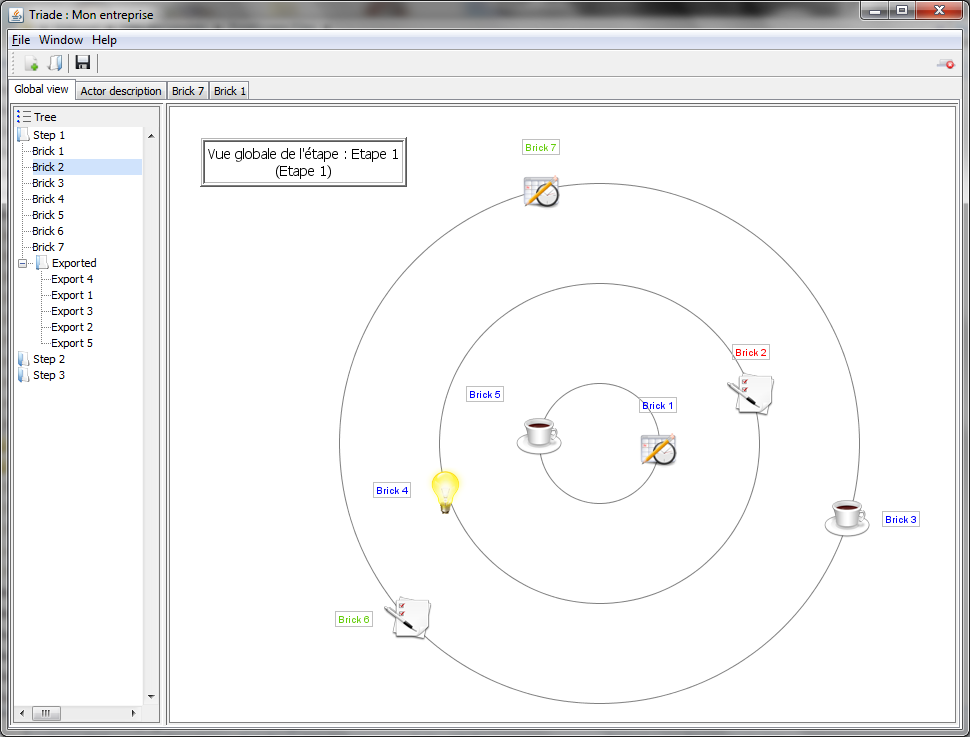
\includegraphics[scale=0.35]{images/vue_globale.png}
\caption{Global view of a step}

\end{figure}

The brick are displayed in three circle in the global view, the closer the bricks is from the center, the more important the role of selected actors is.\\
%Chaque vue globale se présente sous la forme de 3 cercles concentriques. Les briques sont disposés en fonction de l'importance des acteurs sélectionnés par l'utilisateur dans ces briques.
%\begin{itemize}
%\item Dans les briques les plus au centre, les acteurs principaux de l'utilisateur ont un rôle central.
%\item Dans le deuxième cercle, les acteurs principaux ont un rôle secondaire et/ou les acteurs secondaires ont un rôle central ou secondaire.
%\item Dans le troisième cercle les acteurs sélectionnés ont un rôle peu important.\\
%\end{itemize}

The color of brick labels show the state of the relations of the brick :\\
%La couleur des étiquettes des différentes briques indique si les relations de ces briques ont été remplies ou non, et si elles sont en écart. 
\begin{itemize}
\item Blue for incomplete relation.
%\item Le bleu correspond à une brique où des relations n'ont pas été remplies.
\item Red for gapped relation.
%\item Le rouge correspond à une brique où au moins une des relations est en écart.
\item Green for correct relation.\\
%\item Le vert correspond à une brique où toutes les relations sont remplies et aucune ne présente d'écart.
\end{itemize}

If a brick contains incomplete and gapped relation, its label will be blue.\\
%Le rouge étant prioritaire sur le bleu, une brique comportant des relations pas encore remplies et au moins une relation en écart apparaîtra en rouge.\\

You can access to all the exports of a brick by making a right click on his name, or in an empty space in the scheme.\\
%Il est possible d'accéder d'accéder à toutes les exportations réalisée sur une brique en faisant un clic droit sur cette dernière (voir le chapitre \ref{export} sur les exportations).\\

To open a brick, just do a double click on it in the tree or in the global view.\\
%Pour ouvrir une brique, il suffit de faire un double-clic sur son icône dans une vue globale ou sur la ligne de l'arbre correspondante. Un nouvel onglet apparaĩt  pour afficher cette brique. Plusieurs briques peuvent être ouverte en même temps. 

\section{Bricks and relation}
Each brick represent a possible real situation. The different component of the scheme represent the actors, the tools and the activity of the situation.\\
%Chaque brique représente une situation qu'il est possible de rencontrer dans la réalité. Les différents éléments du schéma représente les acteurs, les moyens et l'activité qui composent la brique.\\

\begin{figure}[h!]
\centering
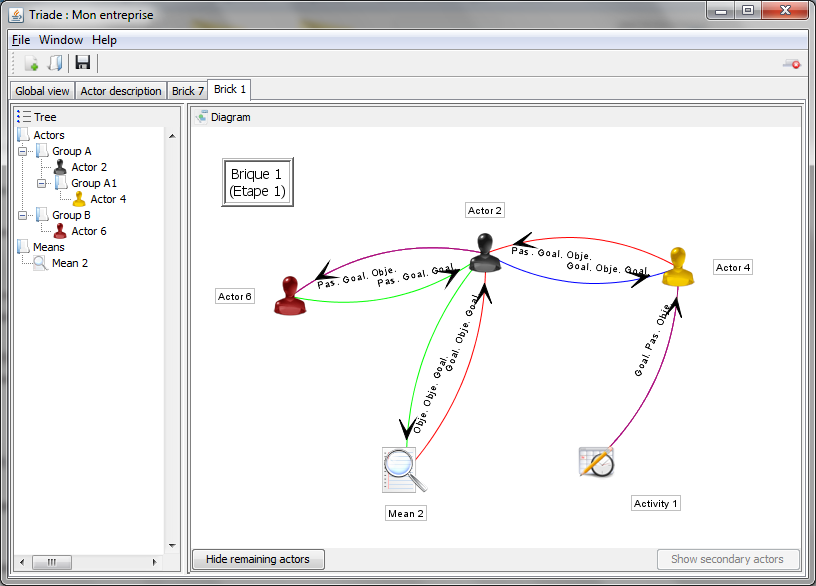
\includegraphics[scale=0.55]{images/brique.png}
\caption{A brick view}

\label{brique}
\end{figure}
When you open a brick for the first time, only the main actors are showned. You have to use the two buttons on the bottom of the window to show more or less actors.\\
%Les éléments apparaissent progressivement afin de permettre à l'utilisateur d'assimiler les différents éléments de la situation. Les deux boutons situés en dessous du schéma permettent d'afficher et de masquer les éléments de la brique.\\

%Les éléments apparaissent dans l'ordre suivant :\\
%\begin{enumerate}
%\item Les moyens, les activités, les acteurs principaux et ceux ayant un rôle central dans la brique.
%\item Les acteurs secondaires et ceux ayant un rôle secondaire.
%\item Les acteurs restants.\\
%\end{enumerate}

A relation between two actors is represented by an arrow from the first actor to the second. The return relation is represented by an opposite arrow (from the second to the first). Those arrow will be sometime called "edge" in this manual.\\
%Les relations entre deux acteurs sont représentées par des flèches entre deux éléments d'un schéma. Ces flèche sont orientées, ainsi une flèche allant d'un acteur A vers un acteur B représente la relation que A a envers B, la relation retour (ie. de B vers A) est associée à la flèche retour.\\

There are two way to select an edge, by clicking on it (or on its label), or by dragging the mouse (while cliking) from the first actor to the second.\\
%Deux manières permettent de sélectionner une arête. Soit en cliquant dessus (ou sur son étiquette), soit en faisant un clic continu à partir du premier acteur jusqu'au deuxième.\\

\begin{figure}[h!]
\centering
\Ovalbox{
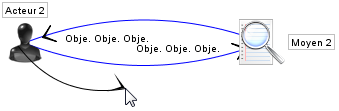
\includegraphics[height=25pt]{images/selection_1.png}
}
\Ovalbox{
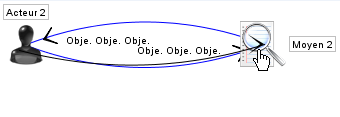
\includegraphics[height=25pt]{images/selection_2.png}
}
\Ovalbox{
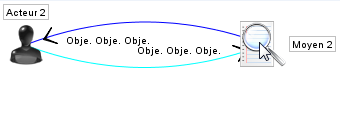
\includegraphics[height=25pt]{images/selection_3.png}
}
\caption{A edge selection by dragging}

\end{figure}

When a relation is selected, a pop-up appears. It allow the user to consult the relation and to fill and modify the real relation. The goals and the meanings for action time could be selection in a list of possibility. The structural relation is showned but it can't be modified.\\
%Lorsqu'on sélectionne une relation, une fenêtre apparaît. Elle permet de consulter et modifier la relation. Il est possible de définir les objectifs et les moyens réels de chaque temps d'action. Une liste de possibilité est fournie pour chaque champ. La relation structurelle est affichée dans cette fenêtre mais ne peut pas être modifiée.\\

The content of an action time could be copied in the next action time by clicking with the button with a down arrow on the left of the line.\\
%La petite flèche située sur la gauche d'un objectif permet de répliquer l'objectif et le moyen réel au temps d'action suivant.

\begin{figure}[h!]
\centering
\Ovalbox{
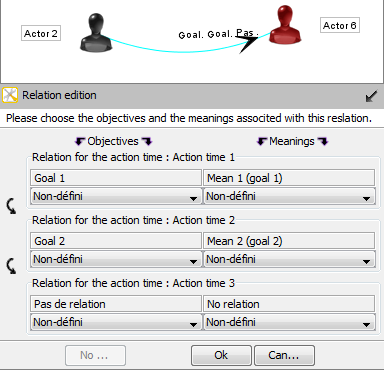
\includegraphics[scale=0.75]{images/edition_relation.png}
}
\caption{Relation edition pop-up}
\label{edition_relation}
\end{figure}

The color of the edge show if the relation is incomplete (blue), gapped (purple for a gap on meanings, red for a gap on goals) or correct (green).\\
%Les relations apparaissent d'une couleur différente en fonction de leur état. Le code couleur utilisé est le même que celui des briques (voir figure~\ref{brique} pour les couleurs des arêtes) :
%\begin{itemize}
%\item Bleu pour une relation incomplète (certains objectifs sont encore à "Non-défini").
%\item Rouge foncé pour une relation en écart au niveau d'un moyen (un des moyens réels est différents du moyen structurel mais les objectifs sont tous en accords).
%\item Rouge clair pour une relation en écart au niveau d'un objectif (un des objectifs réels est en écart, le moyen n'est pas pris en compte).
%\item Vert pour une relation réelle en accord avec la relation structurelle (tous les objectifs et les moyens concordent).
%\end{itemize}

Don't forget to display all actors (with the two buttons on the bottom of the window) in order to see all the relations.\\
%Attention, n'oubliez pas de faire apparaître l'ensemble des acteurs pour avoir accès à toutes les relations d'une brique.\\

Relations are associated to tool-tip which describe entirely the relations. You just have to let the mouse pointer over an edge during 1 second to show the tool-tip.\\
%Les relations sont associées à des info-bulles qui fournissent un résumé complet des objectifs et des moyens de la relation. Il suffit de placer la souris sur une flèche pendant une seconde pour faire apparaître l'info-bulle.\\

It is possible to add an absent relation. But all the structural goals and meanings will be set to "No relation", If the user set all the real relation to "No relation", the edge won't be shown.\\
%Il est possible d'ajouter une relation absente. Cependant, tous les objectifs structurels seront mis à "Pas de relation", de ce fait cette relation sera forcément en écart. Si l'utilisateur définit tous les objectifs réels à "Pas de relation", l'arête ne sera pas affichée.\\

%L'arborescence sur la gauche de la fenêtre présente l'ensemble des acteurs présents dans la brique. Elle permet de sélectionner rapidement un acteur et aussi d'accéder à sa fiche à l'aide d'un clic droit.\\

You can move a vertex with pressing "Shift" in while dragging the vertex. With "Ctrl" you can move the whole scheme.\\
%Il est possible de déplacer un sommet en maintenant la touche "Ctrl" appuyée tout en cliquant sur le sommet. De même pour déplacer l'ensemble des sommets, il faut cliquer sur la touche "Majuscule" (shift) tout en cliquant.\\ 



\section{Default edge label}
It is possible to change the default edge label content. The sub-menu "Brick edge labels" allow the following possibilities : 
%Il est possible de changer le contenu par défaut des étiquettes des arêtes dans les briques. Le sous-menu "Etiquettes des arêtes des briques" dans le menu Edition. Les   différents contenus sont :\\
\begin{itemize}
\item \textbf{Structural relations} : Display the 4 first characters of structural relations for each action times.\\
%\item \textbf{Relations structurelles} : Affiche les 4 premiers caractères des relations structurelles de chaque temps d'action.\\
\item \textbf{Real relations} : The same with real relations.\\
%\item \textbf{Relations réelles} : De même avec les relations réelles.\\
\item \textbf{Relation at action time : *} : Display the structural and the real relations for the selected action time.\\
%\item \textbf{Relation au temps d'action : *} : Affiche la relation structurelle et la relations réelle pour le temps d'action sélectionné.\\ 
\end{itemize}

This setting affect only the edge labels in the bricks. In the exports, edge labels are controlled by the global export settings (see also section \ref{globalExport}).\\
%Cette option ne concerne que les relations dans les briques. Dans les exports, ces étiquettes sont contrôlées par les options globale de l'export (voir paragraphe \ref{globalExport}).\\

\begin{figure}[h!]
\centering
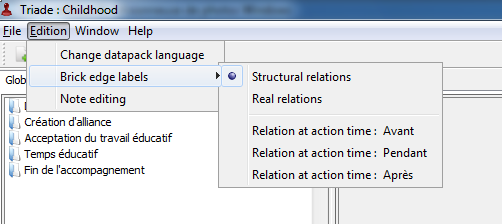
\includegraphics[width=0.5\textwidth]{images/menu_edition.png}
\caption{The default edge label sub-menu}
\label{menu_edition}
\end{figure}


\section{Note editing in bricks}
Each brick is associated with a note. It is useful to keep information and to add some explanation for the situation described in the brick. By default, note are not editable. The option "Note editing" have to be selected to enable note editing. This option is in the edition menu (see picture \ref{menu_edition}). A note is associated to a session, it will be only accessible from the session in which it has been created.\\
%Chaque brique est maintenant associée à une note. Cela permet d'ajouter des informations pour décrire une situation. Par défaut, les notes ne sont pas éditables. Il faut activer l'option "Edition des notes" dans le menu édition avant de pouvoir les modifier (voir image \ref{menu_edition}).\\

Notes are displayed in the upper-right corner of the brick window. The note could be hidden or displayed by clicking on the arrow.\\
%Les notes sont accessibles à l'aide du cadre présent en haut à droite de la zone d'affichage d'une brique. Attention, les notes sont liés à une brique et à une session. En particulier, elles ne sont pas partagées entre les sessions.\\

\begin{figure}[h!]
\centering
\begin{subfigure}{\textwidth}

\centering
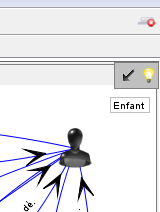
\includegraphics[width=0.4\textwidth]{images/note_fermee.png}
\caption{A note in hidden mode}
\end{subfigure}
\begin{subfigure}{\textwidth}

\centering
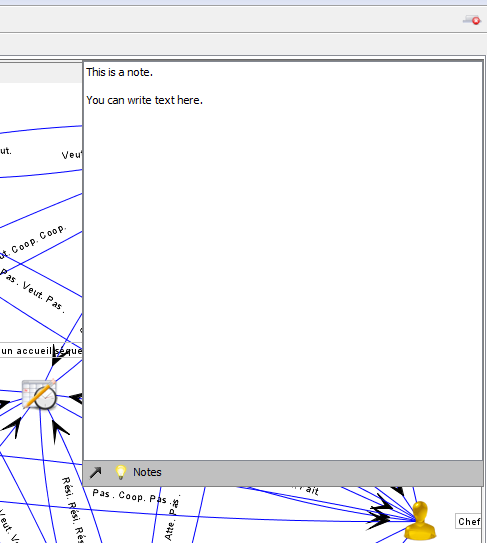
\includegraphics[width=0.4\textwidth]{images/note_ouverte_edition.png}
\caption{An opened note with editing mode enabled}
\end{subfigure}
\begin{subfigure}{\textwidth}

\centering
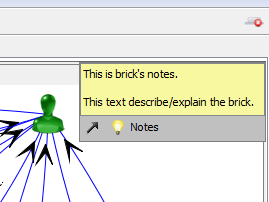
\includegraphics[width=0.4\textwidth]{images/note_ouverte_pas_edition.png}
\caption{An openend note with editing mode disabled}
\end{subfigure}

\end{figure}

